\setAuthor{Päivo Simson}
\setRound{lahtine}
\setYear{2020}
\setNumber{G 5}
\setDifficulty{5}
\setTopic{TODO}

\prob{Solenoid ja kontuur}
Pikka solenoidi läbib muutuva tugevusega vool, mille ajaline sõltuvus on näidatud vasakpoolsel joonisel. Solenoidis on $\SI{1}{cm}$ kohta viis keerdu ning solenoidi teljega ristuvas tasandis paikneb parempoolsel joonisel toodud juhtiv kontuur
	eritakistusega $\rho=\SI{1,7e-8}{\Omega.m}$ ja juhtme ristlõikepindalaga $S_0=\SI{2,5}{mm^2}$. Leidke voolutugevuse maksimaalne väärtus kontuuris. Vaakumi magnetiline läbitavus on $\mu_0=\SI{1.26e-6}{H/m}$.
	
	\begin{center}
		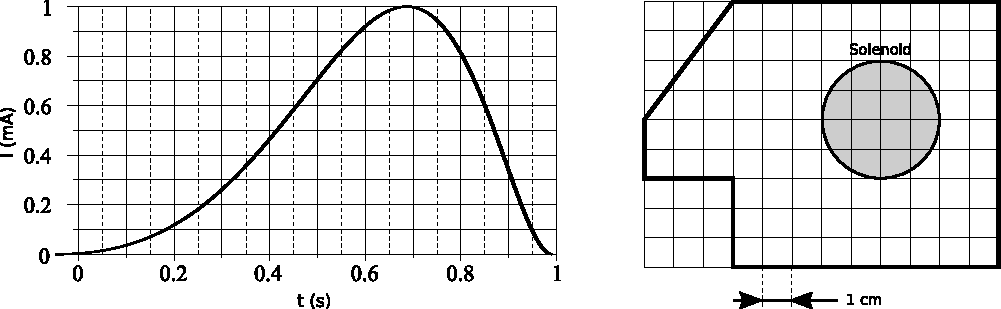
\includegraphics[width=1\linewidth]{2020-lahg-05-yl.pdf}
	\end{center}


	
	
	
	
\hint

\solu
Solenoidi sees on magnetiline induktsioon $B = \mu_0 nI$. Vastavalt Faraday induktsiooniseadusele on kontuuris tekkiv induktsiooni elektromotoorjõud absoluutväärtuselt võrdne kontuuri läbiva magnetvoo $\Phi=BS$ muutumise kiirusega:
\[
\epsilon=\frac{\Delta \Phi}{\Delta t}=S\frac{\Delta B}{\Delta t}=\mu_0 n S \frac{\Delta I_s}{\Delta t},
\]
kus $S=\pi r^2$ on solenoidi ristlõikepindala ja $r$ on ristlõike raadius. Selgitava märkusena olgu öeldud, et elektromotoorjõu vahetu tekitaja on solenoidi ümbritsev pööriselektriväli, mis on tingitud muutuvast magnetväljast solenoidi sees. Elektromotoorjõu tõttu tekib kontuuris vool $I=\epsilon/R =\epsilon S_0/(\rho l)$, kus $l$ on kontuuri pikus.
Tekkiv vool on maksimaalne, kui voolu $I_s$ muutumise kiirus $\Delta I_s/\Delta t$ on absoluutväärtuselt suurim. Funktsiooni $I_s(t)$ graafikult näeme, et see juhtub ajahetkel $t\approx \SI{0,9}{s}$. Vahemikus 
$t=\SI{0.85}{s} \ldots \SI{0.95}{s}$ on $I_s(t)$ graafik ligikaudu sirge ja seega $|\Delta I_s/\Delta t|_{max} \approx (\num{0,6}-\num{0,1})/(\num{0,95}-\num{0,85})=\SI{5}{mA/s}$. Teiselt jooniselt saame solenoidi raadiuse $r=\SI{2}{cm}$ ja kontuuri pikkuse $l=\SI{40}{cm}$. Voolutugevuse maksimaalne väärtus kontuuris on seega
\[
I_{\mathrm{max}}=\frac{\mu_0 \pi r^2 n S_0 }{\rho l}\left|\frac{\Delta I_s}{\Delta t}\right|_{\mathrm{max}}\approx \SI{1,5}{\mu A}.
\]
\probend